\chapter{Test Results}
\section{Reaching a static target}

TODO: la static target se atinge obiectivu de 40 de ori

\begin{table}
    \centering
    \begin{tabular}{|| m{15em} | m{15em} ||}
    \hline \hline
    \strong{Network Configuration} & \strong{Time to complete ($s$)} \\ \hline \hline
    1 layer, 128 units & 183.1415 \\ \hline
    1 layer, 256 units & DNF \\ \hline
    1 layer, 512 units & 205.8087 \\ \hline
    3 layers, 128 units & 182.1884 \\ \hline
    3 layers, 256 units & 180.4801 \\ \hline
    3 layers, 512 units & 180.2796 \\ \hline
    5 layers, 128 units & 170.9822 \\ \hline
    5 layers, 256 units & 186.4627 \\ \hline
    5 layers, 512 units & 205.8265 \\ \hline
    7 layers, 128 units & 188.0436 \\ \hline
    7 layers, 256 units & 182.1618 \\ \hline
    7 layers, 512 units & 219.4408 \\ \hline \hline
    \end{tabular}
    \caption{Test results static course, static brain}
    \label{move_to_static_target_test_results:1}
\end{table}

\begin{figure}
    \begin{center}
        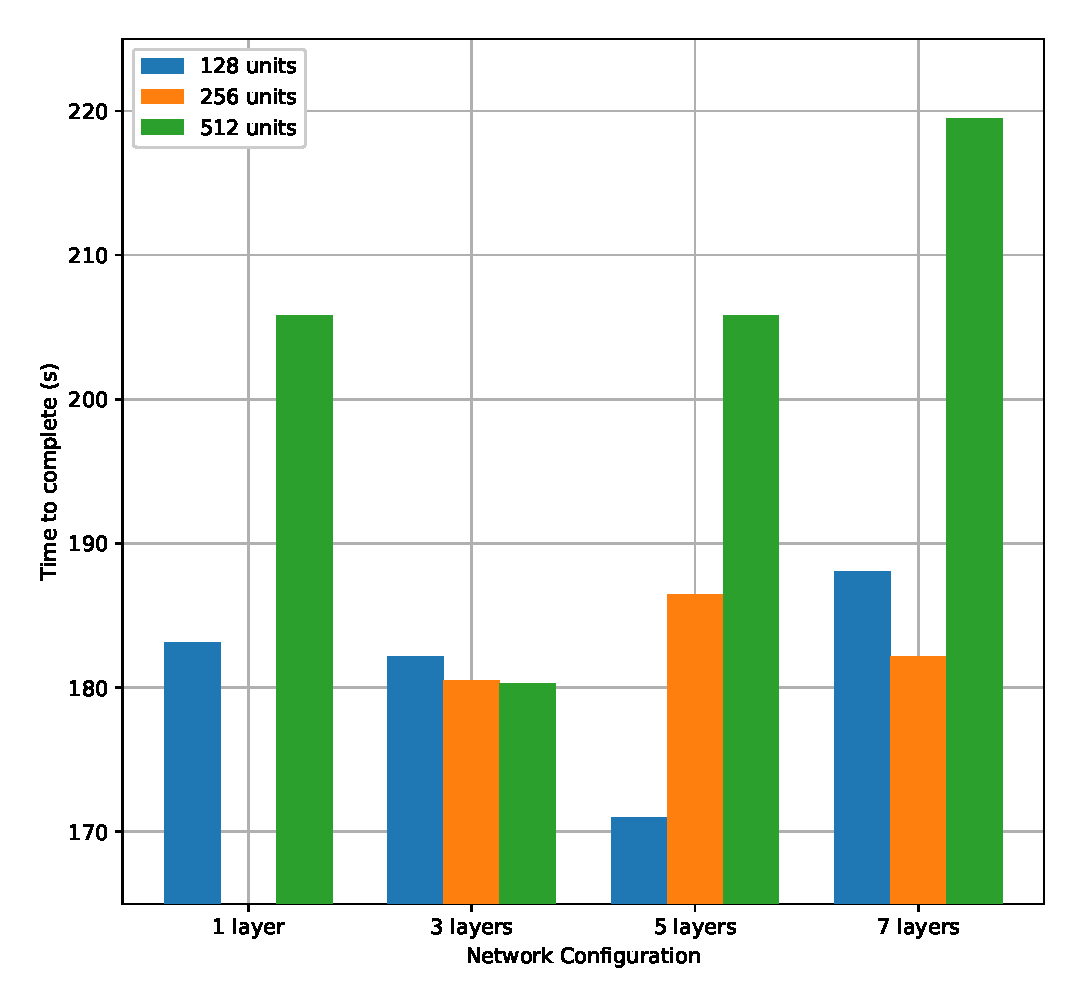
\includegraphics[width=\linewidth]{move_to_static_target_test_static_brain_bar_chart.eps}
        \caption{Test results for static course \& static brain}
        \label{test_results_static_target_static_brain_bar_chart}
    \end{center}
\end{figure}

\begin{table}
    \centering
    \begin{tabular}{|| m{11.3em} | m{10em} | m{9.6em} ||}
    \hline \hline
    \strong{Network Configuration} & \strong{Observed target's direction} & \strong{Time to complete ($s$)} \\ \hline \hline
    1 layer, 128 units & No & 192.7527 \\ \hline
    1 layer, 128 units & Yes & 196.2916 \\ \hline
    1 layer, 256 units & No & 223.6499 \\ \hline
    1 layer, 256 units & Yes & 464.985 \\ \hline
    1 layer, 512 units & No & 215.4364 \\ \hline
    1 layer, 512 units & Yes & 208.1973 \\ \hline
    3 layers, 128 units & No & 200.7101 \\ \hline
    3 layers, 128 units & Yes & 192.2111 \\ \hline
    3 layers, 256 units & No & 291.4421 \\ \hline
    3 layers, 256 units & Yes & 202.1844 \\ \hline
    3 layers, 512 units & No & 321.6053 \\ \hline
    3 layers, 512 units & Yes & 188.5515 \\ \hline
    5 layers, 128 units & No & 252.7738 \\ \hline
    5 layers, 128 units & Yes & 187.1074 \\ \hline
    5 layers, 256 units & No & 363.128 \\ \hline
    5 layers, 256 units & Yes & 215.8631 \\ \hline
    5 layers, 512 units & No & 576.1487 \\ \hline
    5 layers, 512 units & Yes & 214.0343 \\ \hline \hline
    \end{tabular}
    \caption{Test results static course, moving brain}
    \label{move_to_static_target_test_results:2}
\end{table}

\begin{figure}
    \begin{center}
        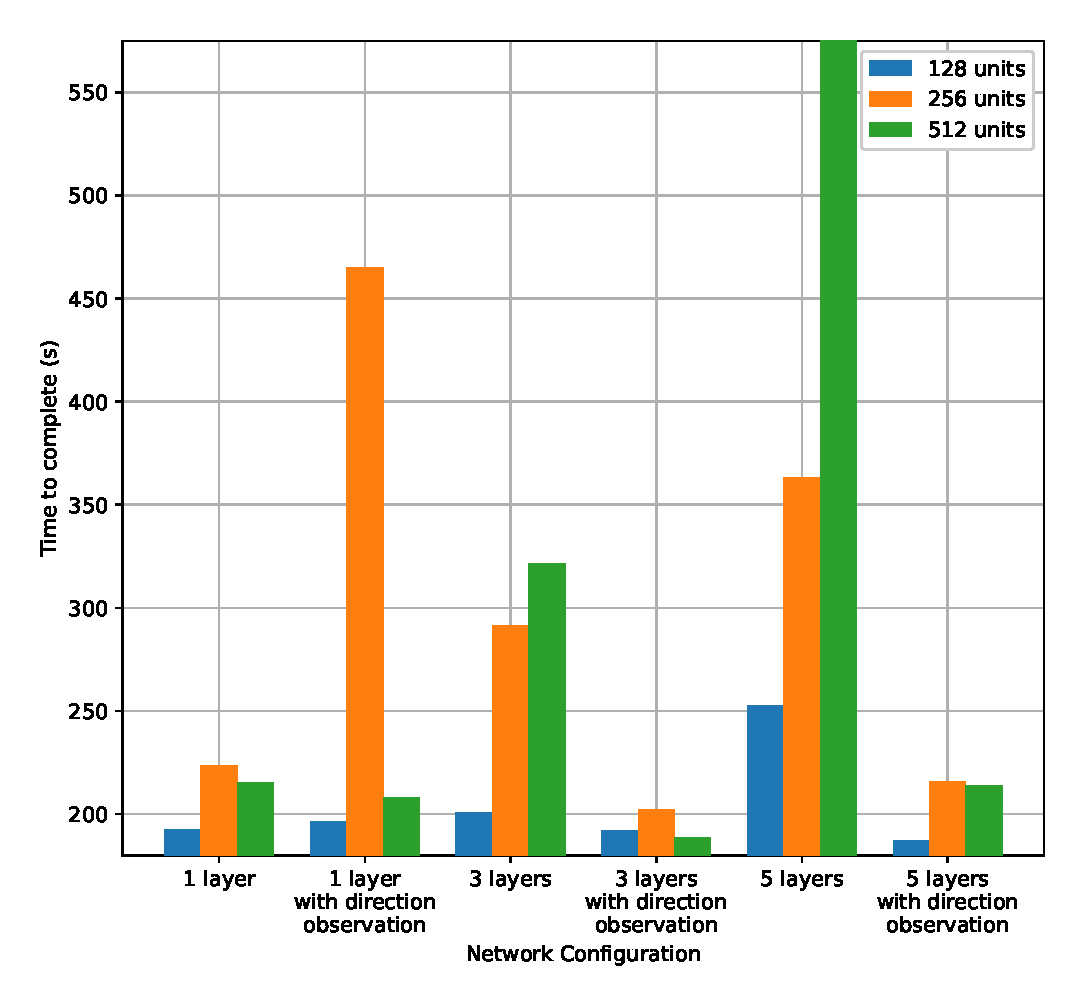
\includegraphics[width=\linewidth]{move_to_static_target_test_moving_brain_bar_chart.eps}
        \caption{Test results for static course \& moving brain}
        \label{test_results_static_target_moving_brain_bar_chart}
    \end{center}
\end{figure}






\section{Reaching a moving target}

TODO: la moving target se atinge obiectivu de 100 de ori


\begin{table}
    \centering
    \begin{tabular}{|| m{15em} | m{15em} ||}
    \hline \hline
    \strong{Network Configuration} & \strong{Time to complete ($s$)} \\ \hline \hline
    1 layer, 128 units & 427.4408 \\ \hline
    1 layer, 256 units & DNF \\ \hline
    1 layer, 512 units & 438.7894 \\ \hline
    3 layers, 128 units & 450.3436 \\ \hline
    3 layers, 256 units & 457.2029 \\ \hline
    3 layers, 512 units & 448.4958 \\ \hline
    5 layers, 128 units & 429.3176 \\ \hline
    5 layers, 256 units & 466.765 \\ \hline
    5 layers, 512 units & 462.7256 \\ \hline
    7 layers, 128 units & 465.1996 \\ \hline
    7 layers, 256 units & 479.0871 \\ \hline
    7 layers, 512 units & 546.0353 \\ \hline \hline
    \end{tabular}
    \caption{Test results moving course, static brain}
    \label{move_to_moving_target_test_results:1}
\end{table}

\begin{figure}
    \begin{center}
        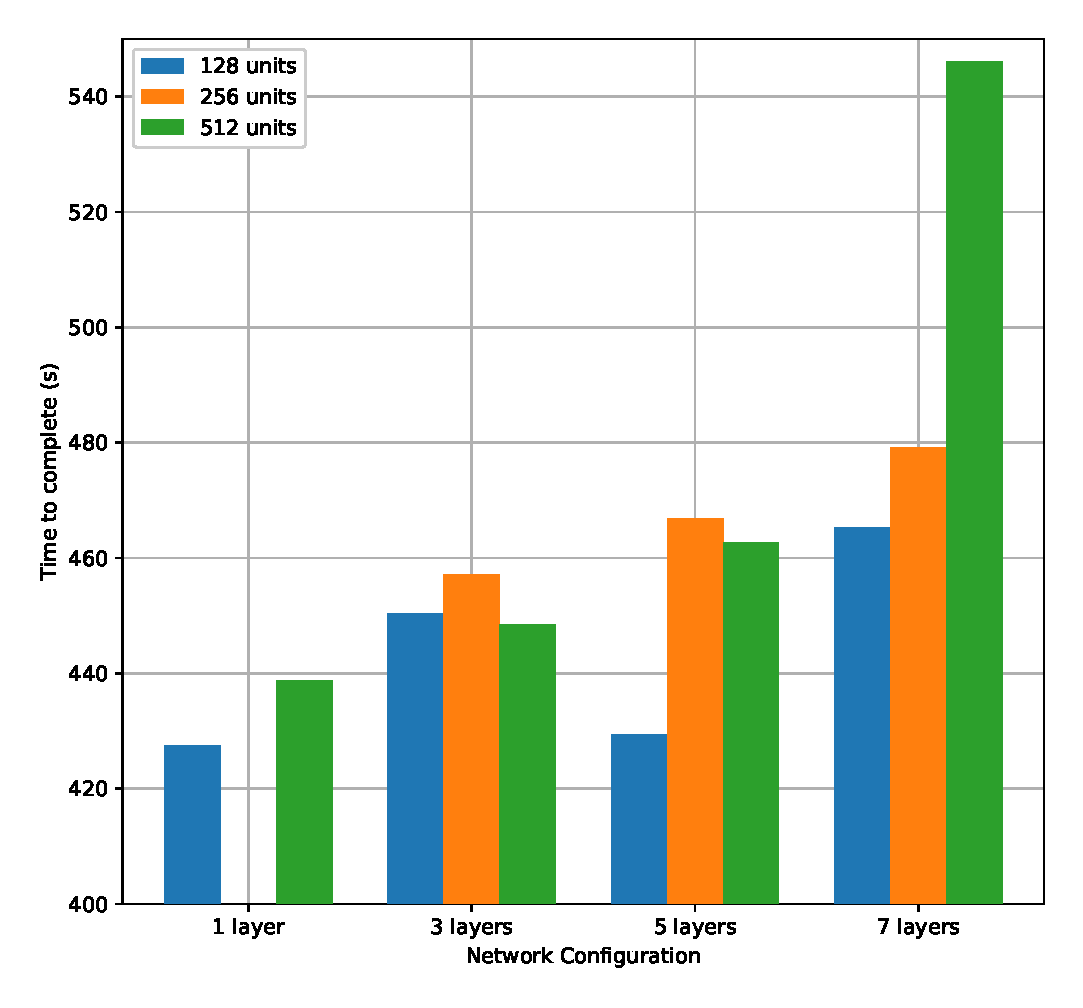
\includegraphics[width=\linewidth]{move_to_moving_target_test_static_brain_bar_chart.eps}
        \caption{Test results for moving course \& static brain}
        \label{test_results_moving_target_static_brain_bar_chart}
    \end{center}
\end{figure}

\begin{table}
    \centering
    \begin{tabular}{|| m{11.3em} | m{10em} | m{9.6em} ||}
    \hline \hline
    \strong{Network Configuration} & \strong{Observed target's direction} & \strong{Time to complete ($s$)} \\ \hline \hline
    1 layer, 128 units & No & 482.4993 \\ \hline
    1 layer, 128 units & Yes & 499.2063 \\ \hline
    1 layer, 256 units & No & 495.7267 \\ \hline
    1 layer, 256 units & Yes & 688.592 \\ \hline
    1 layer, 512 units & No & 452.052 \\ \hline
    1 layer, 512 units & Yes & 485.6294 \\ \hline
    3 layers, 128 units & No & 484.7428 \\ \hline
    3 layers, 128 units & Yes & 488.6792 \\ \hline
    3 layers, 256 units & No & 491.0297 \\ \hline
    3 layers, 256 units & Yes & 485.8719 \\ \hline
    3 layers, 512 units & No & 602.9445 \\ \hline
    3 layers, 512 units & Yes & 467.162 \\ \hline
    5 layers, 128 units & No & 527.4669 \\ \hline
    5 layers, 128 units & Yes & 462.4213 \\ \hline
    5 layers, 256 units & No & 549.7428 \\ \hline
    5 layers, 256 units & Yes & 500.7562 \\ \hline
    5 layers, 512 units & No & 568.0677 \\ \hline
    5 layers, 512 units & Yes & 506.722 \\ \hline \hline
    \end{tabular}
    \caption{Test results moving course, moving brain}
    \label{move_to_moving_target_test_results:2}
\end{table}

\begin{figure}
    \begin{center}
        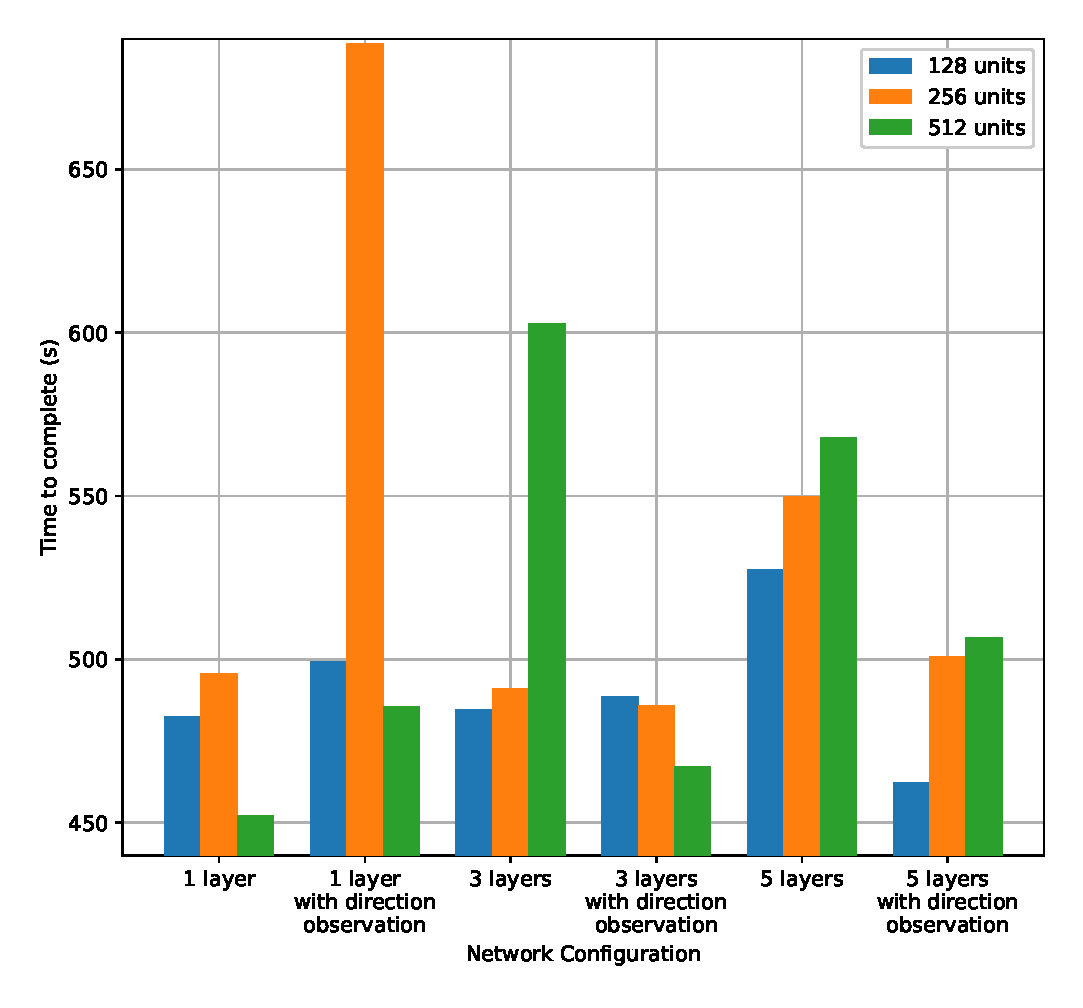
\includegraphics[width=\linewidth]{move_to_moving_target_test_moving_brain_bar_chart.eps}
        \caption{Test results for moving course \& moving brain}
        \label{test_results_moving_target_moving_brain_bar_chart}
    \end{center}
\end{figure}


\section{Shooting a moving target}

TODO: la shooting target se impusca obiectivu de 100 de ori

\begin{table}
    \centering
    \begin{tabular}{|| m{15em} | m{15em} ||}
    \hline \hline
    \strong{Network Configuration} & \strong{Time to complete ($s$)} \\ \hline \hline
    1 layer, 128 units & 499.8927 \\ \hline
    1 layer, 256 units & 564.696 \\ \hline
    1 layer, 512 units & 536.6353 \\ \hline
    3 layers, 128 units & 590.7621 \\ \hline
    3 layers, 256 units & 637.085 \\ \hline
    3 layers, 512 units & 736.3587 \\ \hline
    5 layers, 128 units & 606.5751 \\ \hline
    5 layers, 256 units & 675.0099 \\ \hline
    5 layers, 512 units & 817.632 \\ \hline
    7 layers, 128 units & 837.6456 \\ \hline
    7 layers, 256 units & 872.1839 \\ \hline
    7 layers, 512 units & 914.4853 \\ \hline \hline
    \end{tabular}
    \caption{Final training results}
    \label{shoot_moving_targets_test_results:1}
\end{table}

\begin{table}
    \centering
    \begin{tabular}{|| m{11.5em} | m{12em} | m{10em} ||}
    \hline \hline
    \strong{Network Configuration} & \strong{Bullet Observations} & \strong{Time to complete ($s$)} \\ \hline \hline
    1 layer, 128 units & Bullet's direction and speed & 528.1937 \\ \hline
    1 layer, 128 units & Bullet's speed & 547.2708 \\ \hline
    1 layer, 128 units & Only if bullet was fired & 499.8927 \\ \hline
    3 layers, 128 units & Bullet's direction and speed & 529.0487 \\ \hline
    3 layers, 128 units & Bullet's speed & 557.6132 \\ \hline
    3 layers, 128 units & Only if bullet was fired & 590.7621 \\ \hline
    5 layers, 128 units & Bullet's direction and speed & 628.6615 \\ \hline
    5 layers, 128 units & Bullet's speed & 688.095 \\ \hline
    5 layers, 128 units & Only if bullet was fired & 606.5751 \\ \hline
    7 layers, 128 units & Bullet's direction and speed & 687.3325 \\ \hline
    7 layers, 128 units & Bullet's speed & 684.9317 \\ \hline
    7 layers, 128 units & Only if bullet was fired & 837.6456 \\ \hline \hline
    \end{tabular}
    \caption{Final training results with observation comparasion}
    \label{shoot_moving_targets_test_results:2}
\end{table}


\begin{figure}
    \begin{center}
        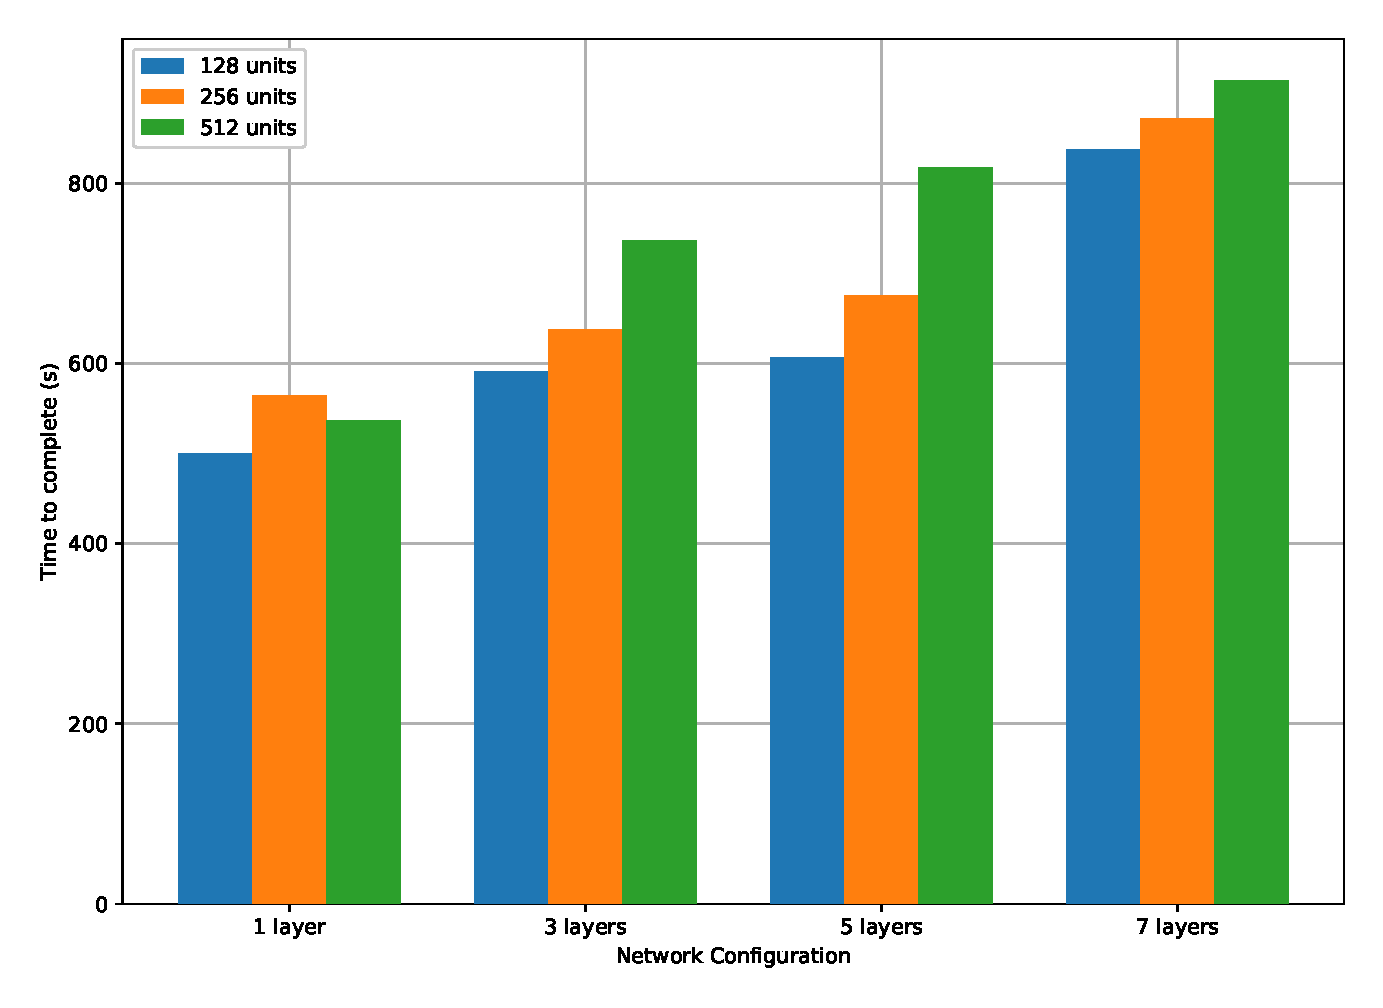
\includegraphics[width=\linewidth]{shoot_moving_target_test_bar_chart.eps}
        \caption{Test results for shooting a moving target}
        \label{test_results_shoot_moving_target_bar_chart}
    \end{center}
\end{figure}

\begin{figure}
    \begin{center}
        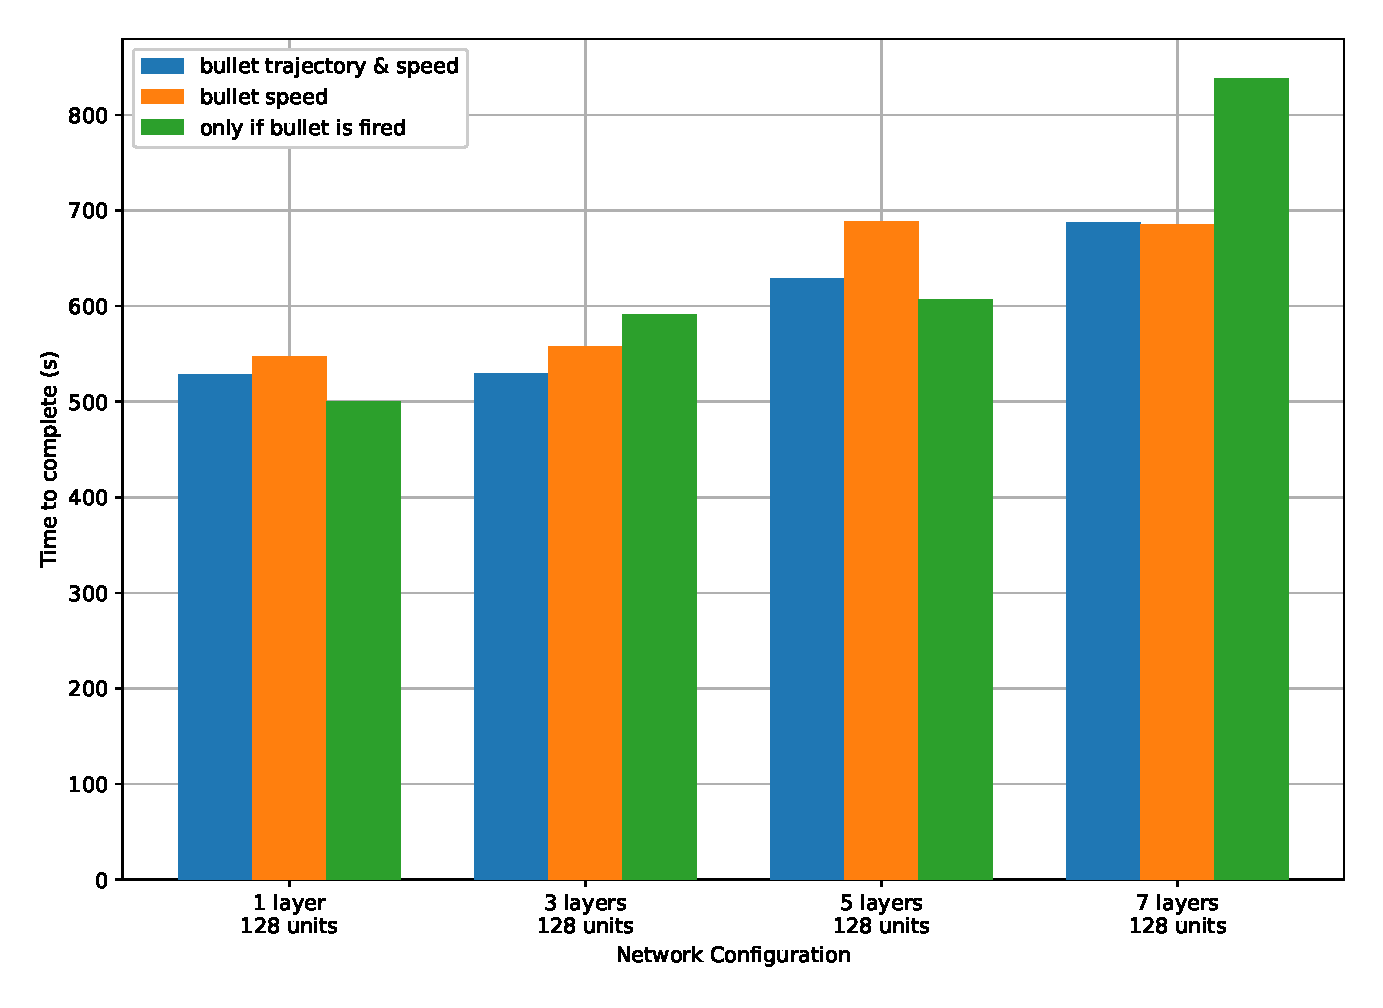
\includegraphics[width=\linewidth]{shoot_moving_target_test_obs_comparasion_bar_chart.eps}
        \caption{Test results for shooting a moving target based on bullet observations}
        \label{test_results_shoot_moving_target_obs_comparasion_bar_chart}
    \end{center}
\end{figure}